\subsection{Single Camera Testing}
After obtaining two of the MT9V034 cameras chosen through the process described in Section \ref{camdecision}, several steps were taken to obtain test images from each camera. These steps are outlined in the following sections.
\par
According to the MT9V034 datasheet, each camera module needed to be supplied with an external Master Clock and Output Enable signal in order to operate \cite{mt9v034}. A simple Verilog module for the Nexys3 Spartan-6 FPGA board was created that supplied the camera module with a 24MHz master clock signal, and a switch was used to toggle the output enable line. With this module implemented, the camera module's default outputs were then observed. In order to interface the camera module with an FPGA, the breakout board shown in Figure \ref{camBreakoutBoard} was also designed to make the module's pins more easily accessible. 

\begin{figure}[H]
	\centerline{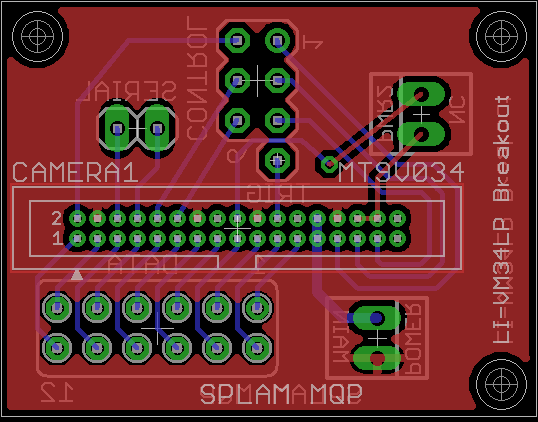
\includegraphics[width=0.5\textwidth]{camera_board.png}}
	\caption{LI-VM34LP Breakout Board}
	\label{camBreakoutBoard}
\end{figure}

\subsubsection{I$^2$C Control} 
Although the MT9V034 camera's I$^2$C control registers were closed source, the previous model's register settings were found to work with the current model  \cite{mt9v032}. As a baseline, the camera module was sent a read request at address 0x00, which should have returned 0x1324 for the MT9V034 camera module. An oscilloscope screenshot of this request is shown in Figure \ref{camVersion}, where the first packet consisted of a request to address 0x00 of device 0x058, and the second packet consisted of the camera's response of 0x1324.
\begin{figure}[H]
	\centerline{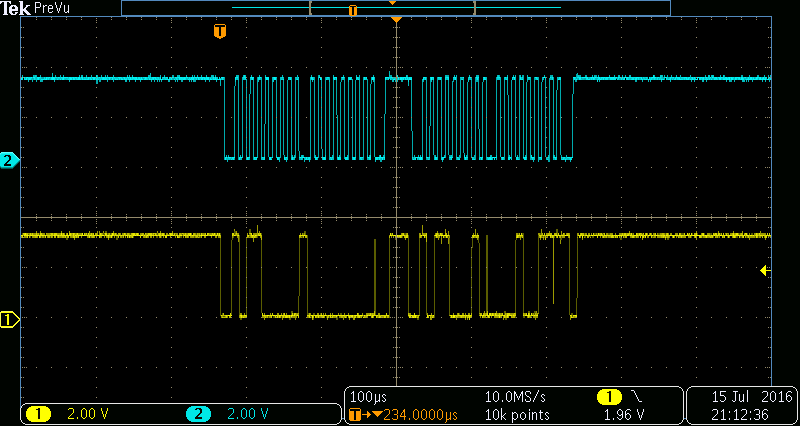
\includegraphics[width=1.0\textwidth]{oScope/i2c_0x00/tek00001.png}}
	\caption{Example I$^2$C Transfer with Camera}
	\label{camVersion}
\end{figure}

\par
After the camera I$^2$C was deemed working, the camera control register was modified to put the camera in "snapshot" mode. In this mode, the camera module no longer continuously took pictures, and only gathered new images when an external trigger was activated. This was the mode in which each camera needed to operate to acquire stereo imagery, since a shared trigger line allowed for both cameras to be controlled simultaneously.
\par
According to the previous camera model's datasheet, the camera module's operational mode was set using control register 0x07. By default, this register was set to a value of 0x0388, which corresponded to master mode with parallel output and simultaneous readout of pixel data enabled \cite{mt9v032}. The camera was placed in trigger mode by writing the control register with value 0x0198, which allowed for the same functionality as before with the exception of having continuous shutter mode replaced with an external trigger. For reference, a table with camera control register bit descriptions can be found in Appendix item \ref{camctlreg} \cite{mt9v032}.
\par
A button input was then attached to the camera's TRIGGER input line, and the TRIGGER and FRAME\_VALID lines were observed on channels one and two of the oscilloscope, as shown in Figure \ref{camInTrigMode}. This oscilloscope screenshot demonstrated that the camera was no longer in continuous operation, since FRAME\_VALID only asserted itself in response to a TRIGGER input. 
\begin{figure}[H]
	\centerline{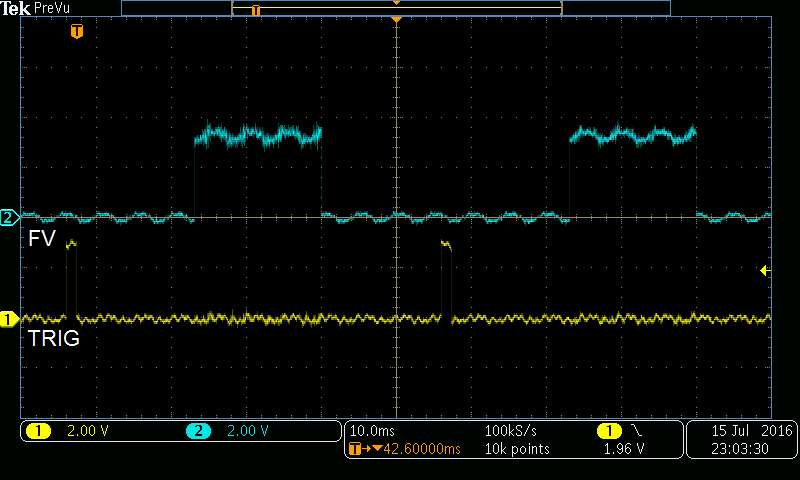
\includegraphics[width=1.0\textwidth]{oScope/i2c_0x07/externalTrigger/externalTrig.png}}
	\caption{Camera Trigger and FV in Trigger Mode}
	\label{camInTrigMode}
\end{figure}
\par
In order to prevent accidental modification of the camera module's configuration registers, the register lock feature of the camera I$^2$C bus was also used. By writing 0xDEAD to register 0xFE, the camera's I$^2$C write functionality was disabled. This feature was disabled when 0xBEEF was written to the register lock register, or when the power of the device was cycled.
\subsubsection{Data Management} 
After a camera control interface was created that placed the MT9V034 camera module in trigger mode, image data was then acquired from the module for viewing. The included AL422B FIFO IC made it so that all triggered imagery was captured and stored external to the FPGA, and allowed for image data to be read in non-continuous chunks. Keeping this in mind, the system shown in Figure \ref{camTestBDG} was created for capturing, storing, and transmitting camera images to a computer for external analysis. Development time of this system was reduced by including an external microcontroller for controlling the camera module's I$^2$C control interface. Various buttons and switches on the FPGA controlled the camera output and trigger, and allowed for a user to trigger an image for storage on the AL422B FIFO. Once the image had been stored on the FIFO, the FPGA read the image line-by-line into an internal buffer. An internal System on Chip (SoC) microcontroller controlled FPGA reads from the FIFO into this internal buffer. An image dump would begin when the SoC microcontroller signaled to the FPGA to read a new line of pixels into its internal 8-bit by 752-address pixel buffer. The FPGA then signaled to the microcontroller when this buffer was full, and the microcontroller would print out the value of each pixel in the buffer to a connected computer over a Universal Asynchronous Reciever/Transmitter (UART) port. When the microcontroller finished printing out the value of each pixel in the line buffer, it signaled to the FPGA to read in a new line of pixels. This process repeated for each of the 480 lines of pixels in the image, and allowed for the transmission of an entire image's worth of data from FIFO to computer. The Verilog implementation of the top module and line buffer for this interface are located in Appendix item \ref{mt9v034TestCode}.

\begin{figure}[H]
	\centerline{\includegraphics[width=1.0\textwidth]{camTestBlockDiag.png}}
	\caption{Camera Test System Block Diagram}
	\label{camTestBDG}
\end{figure}
\par
An example of the transmission of one line of pixel data from the FIFO to the FPGA is shown in Figure \ref{fifoDataOut}.  The green, purple, blue, and yellow lines in this image represent pixel data, FIFO read enable, read reset, and read clock, respectively. Since the FPGA read in one line of pixel data at a time, this process took 752 read clock cycles, as measured in Figure \ref{fifoDataOut}. An internal counter and seven-segment display controller were also implemented on the FPGA to simplify debugging, and displayed a running count of the number of pixel lines that were read into the FPGA's internal buffer, ranging from 0x0000-0x01E0 (0-480). 
\begin{figure}[H]
	\centerline{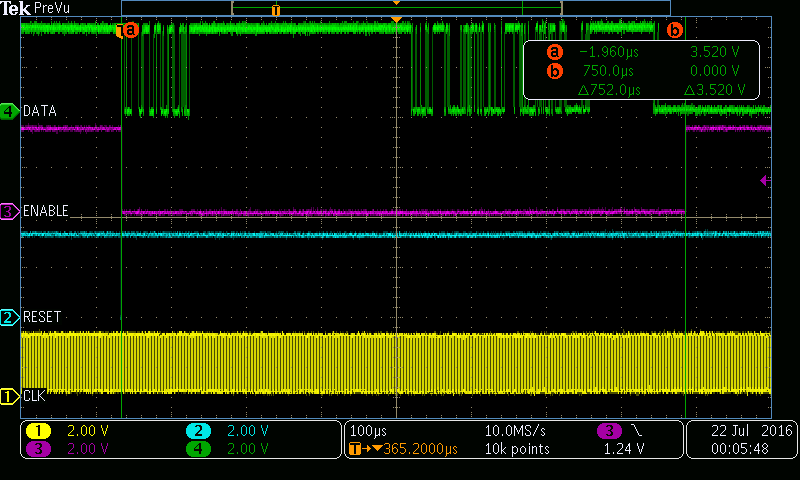
\includegraphics[width=1.0\textwidth]{oScope/camera_fifo/fifo_rstAndDataTimed.png}}
	\caption{Transferring Line Data from FIFO to FPGA}
	\label{fifoDataOut}
\end{figure}

\subsubsection{Transmitting Images Over UART for Analysis} \label{UARTimg}
Once the FIFO and FPGA line buffer interfaces were created, the source code found in Appendix item \ref{camTestC} was implemented on a Microblaze SoC that transmitted camera line data from the FPGA's internal line buffer to an attached computer over UART. An example of the microcontroller's UART output is shown in Figure \ref{PuTTYfifoData}. The microcontroller printed the value of each pixel followed by a newline and carriage return, starting with the top left pixel in the acquired image. 
\begin{figure}[H]
	\centerline{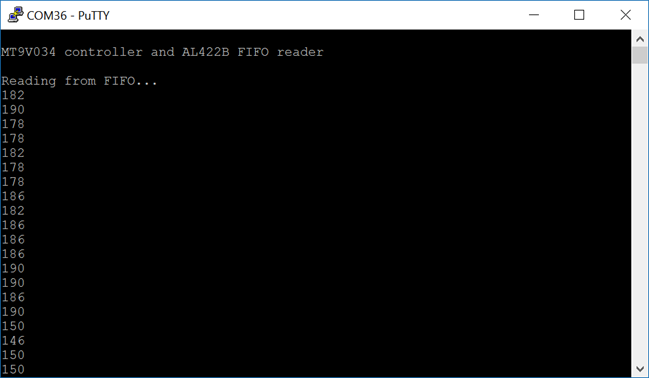
\includegraphics[width=0.8\textwidth]{oScope/camera_fifo/PuTTy.png}}
	\caption{Reading FIFO Data}
	\label{PuTTYfifoData}
\end{figure}
\par
After the image was received through PuTTy, the \textsc{Matlab} script found in Appendix item \ref{camTestMatlab} was used to parse the corresponding logfile into a greyscale image. An example image created through this process is shown in Figure \ref{notebookImage}. Note that the sub-optimal quality of this image was due to signal interference and degradation in the test setup's long wiring, as shown in Figure \ref{camTestSetup}. 
\begin{figure}[H]
	\centerline{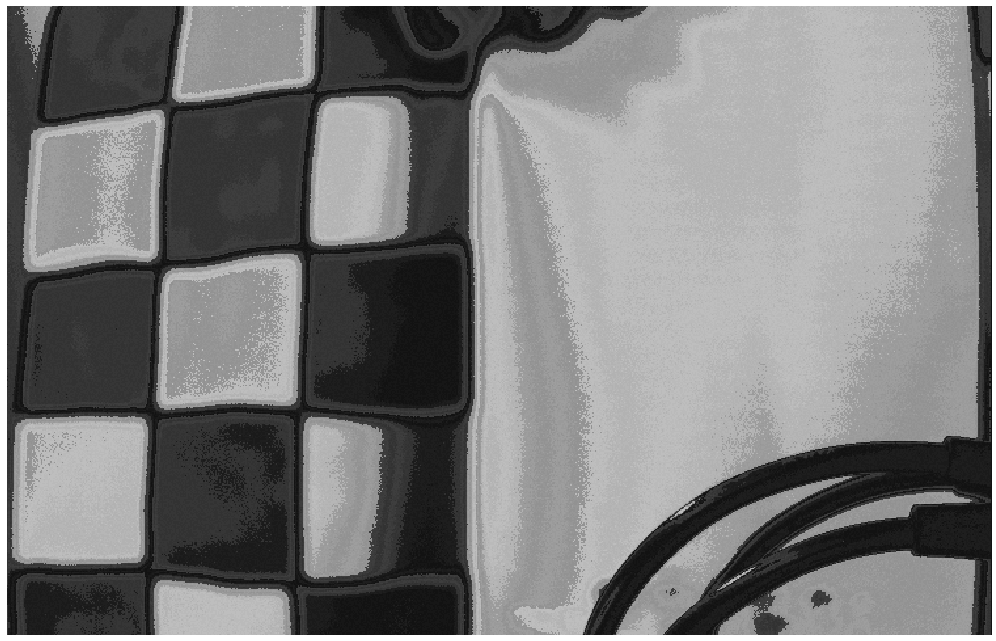
\includegraphics[width=0.75\textwidth]{oScope/camera_fifo/notebook.png}}
	\caption{Notebook With Grid and Oscilloscope Leads}
	\label{notebookImage}
\end{figure}
\par
Although this system was tested using the Nexys3 (Spartan-6) FPGA board, the use of an external FIFO and little to no platform-specific hardware made it so that it could easily be implemented on any system, including the Zynq family of processors that were used in the final system implementation.   
\begin{figure}[H]
	\centerline{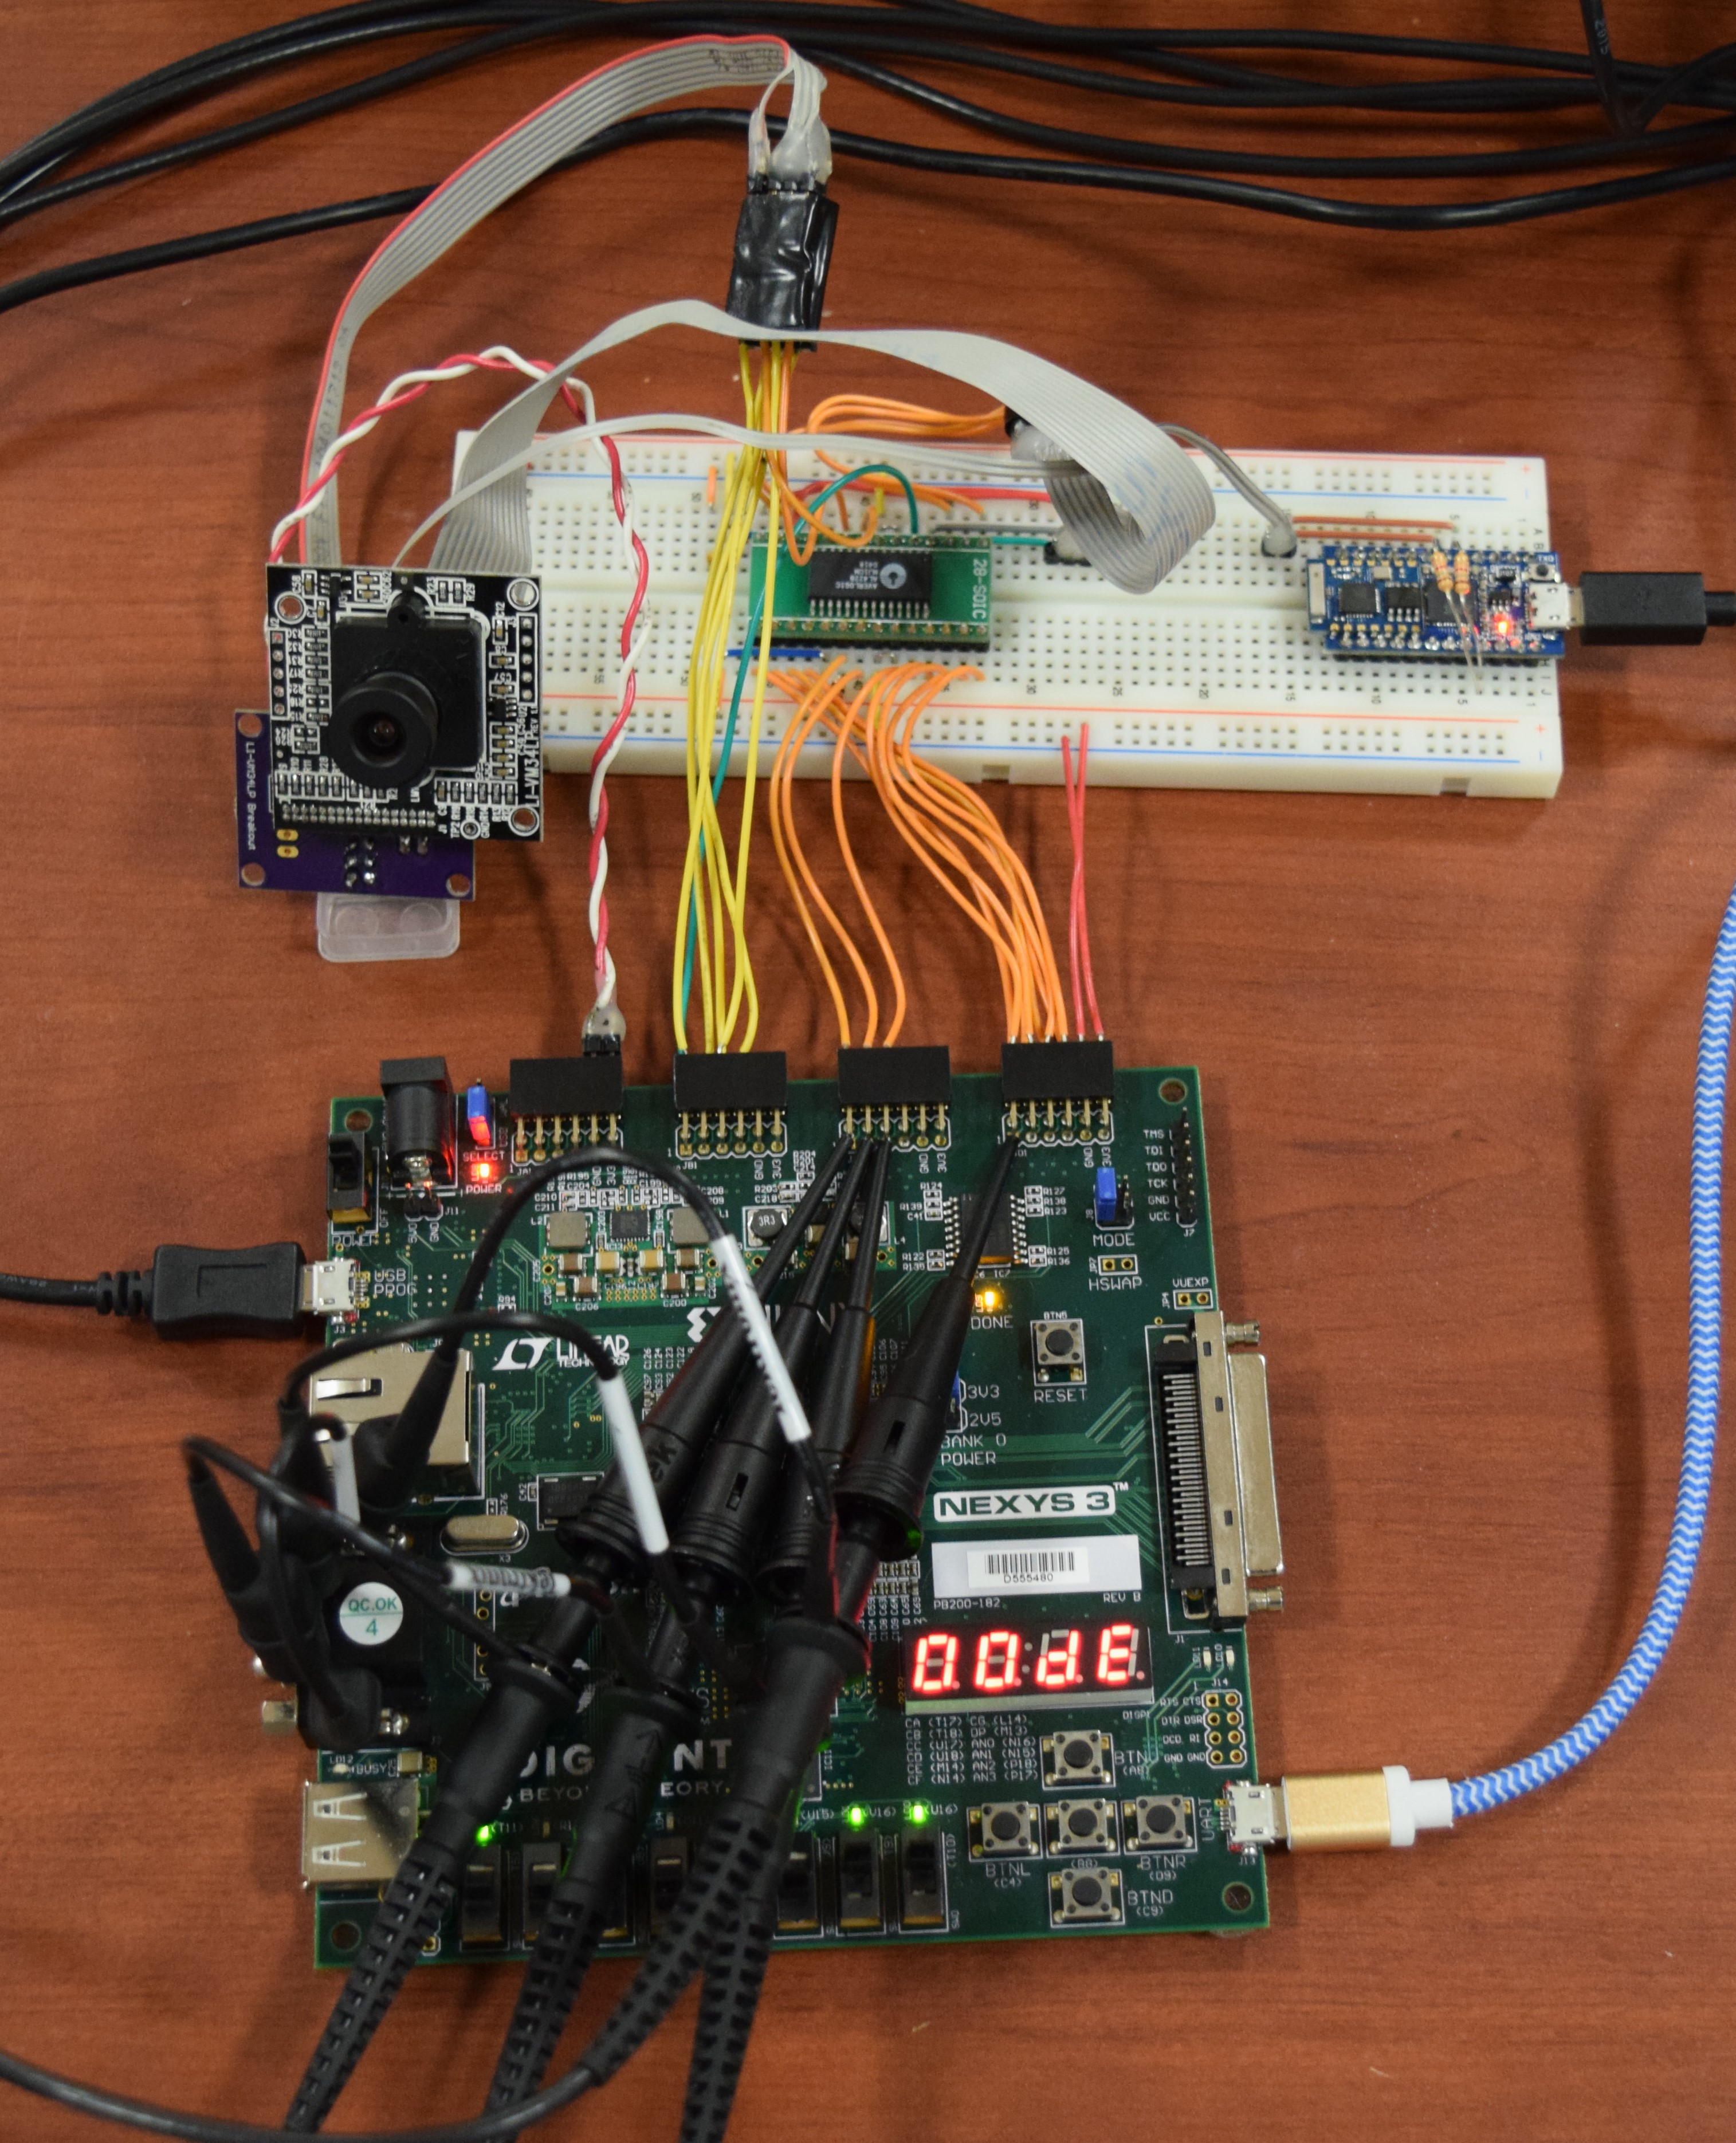
\includegraphics[width=0.75\textwidth]{oScope/camera_fifo/camTestSetup.jpg}}
	\caption{Camera Test Setup}
	\label{camTestSetup}
\end{figure}

\subsection{Final Camera Hardware Implementation}
After successfully gathering image data from a single camera module, an interface was created for controlling both cameras at once using the ZedBoard. This implementation had several design constraints, as it needed to successfully interface both cameras with the ZedBoard as a stereo pair without consuming too many IO pins. 
\subsubsection{Stereo Camera Breakout Board}
Although it was possible to interface each camera module directly to the ZedBoard's GPIO using the camera breakout boards described earlier, this setup was not feasible. A pair of the original camera breakout boards shown in Figure \ref{camBreakoutBoard} would have consumed every available Pmod pin on the board, leaving no additional pins for the IMU or rangefinder\footnote{$[2*(D[9:0]+TRIGGER+OE+RST+SCLK+PCLK+FV+LV)]+SDA+SCL = 36\,\,pins$}. One solution originally investigated was the use of the ZedBoard's FPGA Mezzanine Card (FMC) connector, since it contained 68 available GPIO pins and would have been more than adequate for interfacing the stereo cameras with the board. However, the FMC connector was configured to provide logic voltage levels of only 1.8 or 2.5 volts without modification to the ZedBoard. Since each camera module was only compatible with 3.3 volt logic, the FMC connector was therefore not feasible for our designs.
\par
This left the final option of reducing the overall pin count required by the cameras and interfacing the combined camera setup with the board's Pmod pins. One significant method used for reducing the necessary pins required was to include an individual AL422B FIFO per camera. Based on the testing described in the previous section, it was already determined that these FIFO modules were compatible with the MT9V034 cameras, that they significantly reduced FPGA memory and timing requirements. A second major advantage of including these FIFO modules in the camera interface was that their data output lines supported being placed in a high-impedance state. This meant that the individual data output lines of each FIFO module could be connected in parallel, with a single FIFO driving the lines at a time. Since the bulk of each camera module's required pin count lay in its data lines, the ability to connect these lines in parallel reduced the overall camera GPIO requirements by 8 pins. Since each AL422B FIFO module was capable of being read from at a clock speed of up to 50MHz and the maximum master clock rate of each MT9V034 camera module was 27MHz, the inclusion of the FIFO modules also didn't cause a significant decrease in the overall speed of the stereo camera system \cite{al422b,mt9v034}.
\par
Along with the shared camera data lines between each AL422B FIFO module, it was also possible to connect several other signals in parallel. Since each camera image capture needed to be triggered at approximately the same time for an stereo imaging setup, it was already desirable to connect both camera TRIGGER lines together. The RST, OE, SDL, SCA, and SCLK lines of each camera module were also tied together in pairs of two, and the OE lines were held at 3.3 volts. Lastly, since each camera LV signal needed to be inverted for use with the AL422B FIFOs, a discrete inverter IC was used to save on FPGA GPIO. Overall, these modifications saved a total of 25 pins, as shown in Equation \ref{lowerPincount}.
\begin{equation}
\label{lowerPincount}
\begin{split}
36\,\, Pins - (8\,\,Data + 4 \,\,truncated\,\,bits) - (TRIGGER+SCLK+RST) \\ - 2*(OE+PCLK+FV+LV) = 13\,\,pins\,(!) 
\end{split}
\end{equation}
\par
Note that each FIFO needed to be controlled individually, requiring an additional Read Reset (RRST) and Read Enable (RE) pin per camera, as well as a shared Read Clock (RCK) line. This brought the total pin count required by the stereo camera setup to 16 pins plus two I\textsuperscript{2}C pins, which was conveniently the number of GPIO available in two Pmod headers. This setup was implemented as shown in Appendix item \ref{stereoCameraSchematic}, and the final stereo camera breakout board shown in Figure \ref{stereoCameraBoard} was then created.  
\par
A Verilog module was created using a modified version of the MT9V034 camera test code found in Appendix item \ref{mt9v034TestCode} that tested the stereo camera breakout board's functionality using the Nexys3 platform. A switch input selected one of the two camera modules for image acquisition, and a binned 60x92 pixel set from the center of the camera's image was buffered locally for an attached VGA display. The image was then independently written to the display according to VGA pixel timing. This process was repeated at a high rate of speed, and allowed for a real-time video stream from the selected camera to be displayed. The assembled stereo breakout board used in this test is shown in Figure \ref{stereoTestSetup}.
\begin{figure}[H] 
	\begin{subfigure}{1\textwidth}
	\centering
		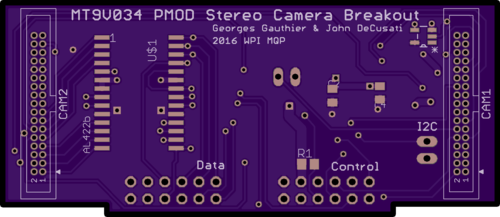
\includegraphics[width=0.65\linewidth]{stereo_top.png}
		\caption{PCB Top}
	\end{subfigure}
	\begin{subfigure}{1\textwidth}
	\centering
		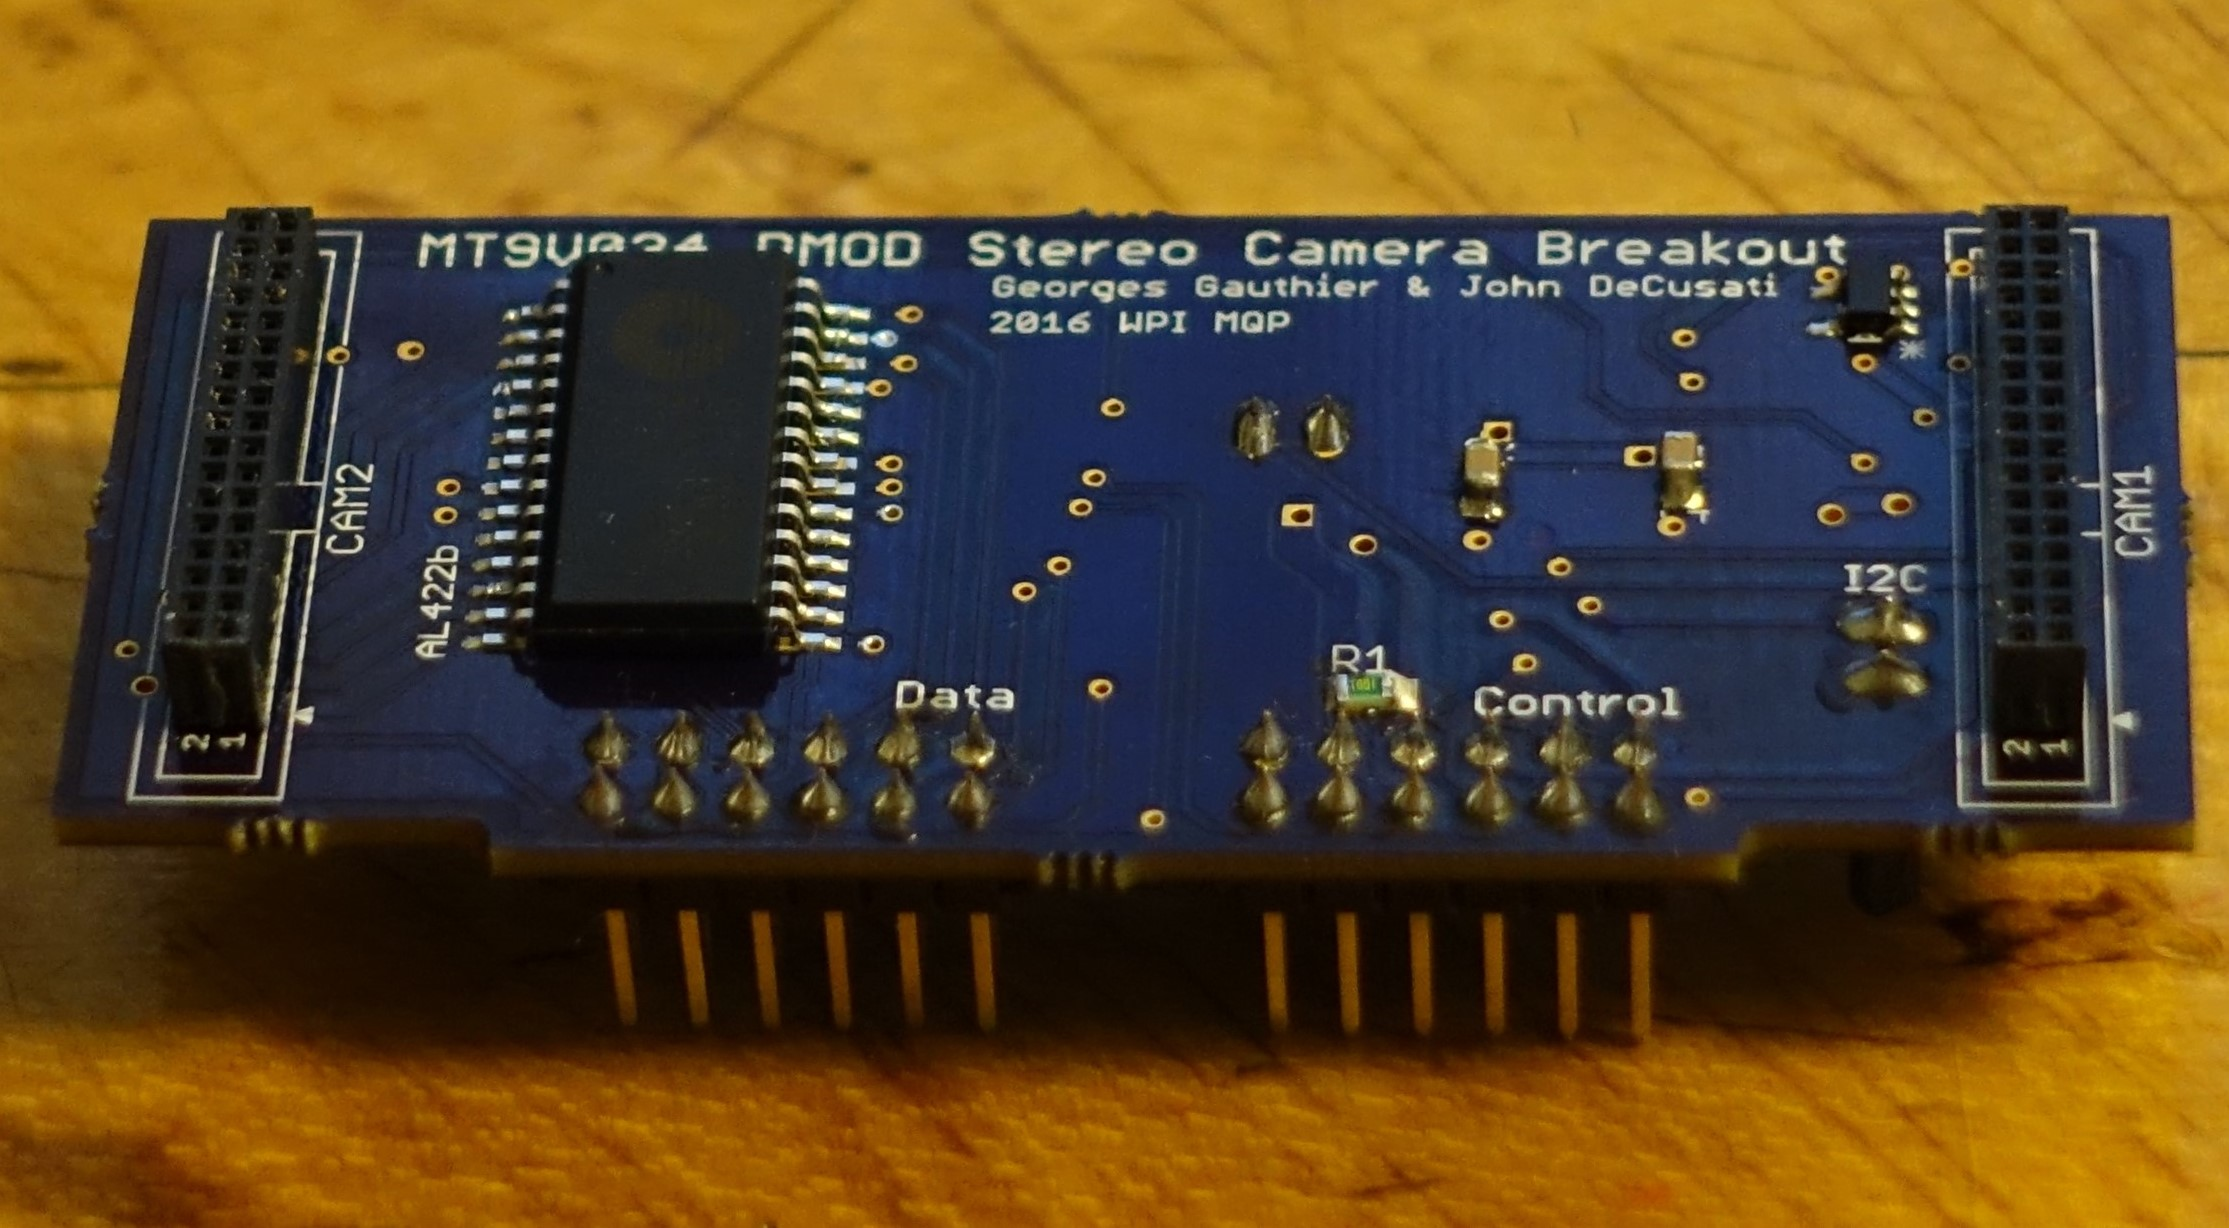
\includegraphics[width=0.65\linewidth]{stereo_board_assembled.JPG}
		\caption{Assembled PCB}
	\end{subfigure}
	\caption{Stereo Camera Pmod PCB}
	\label{stereoCameraBoard}
\end{figure}
\par
\begin{figure}[H] 
	\centering
	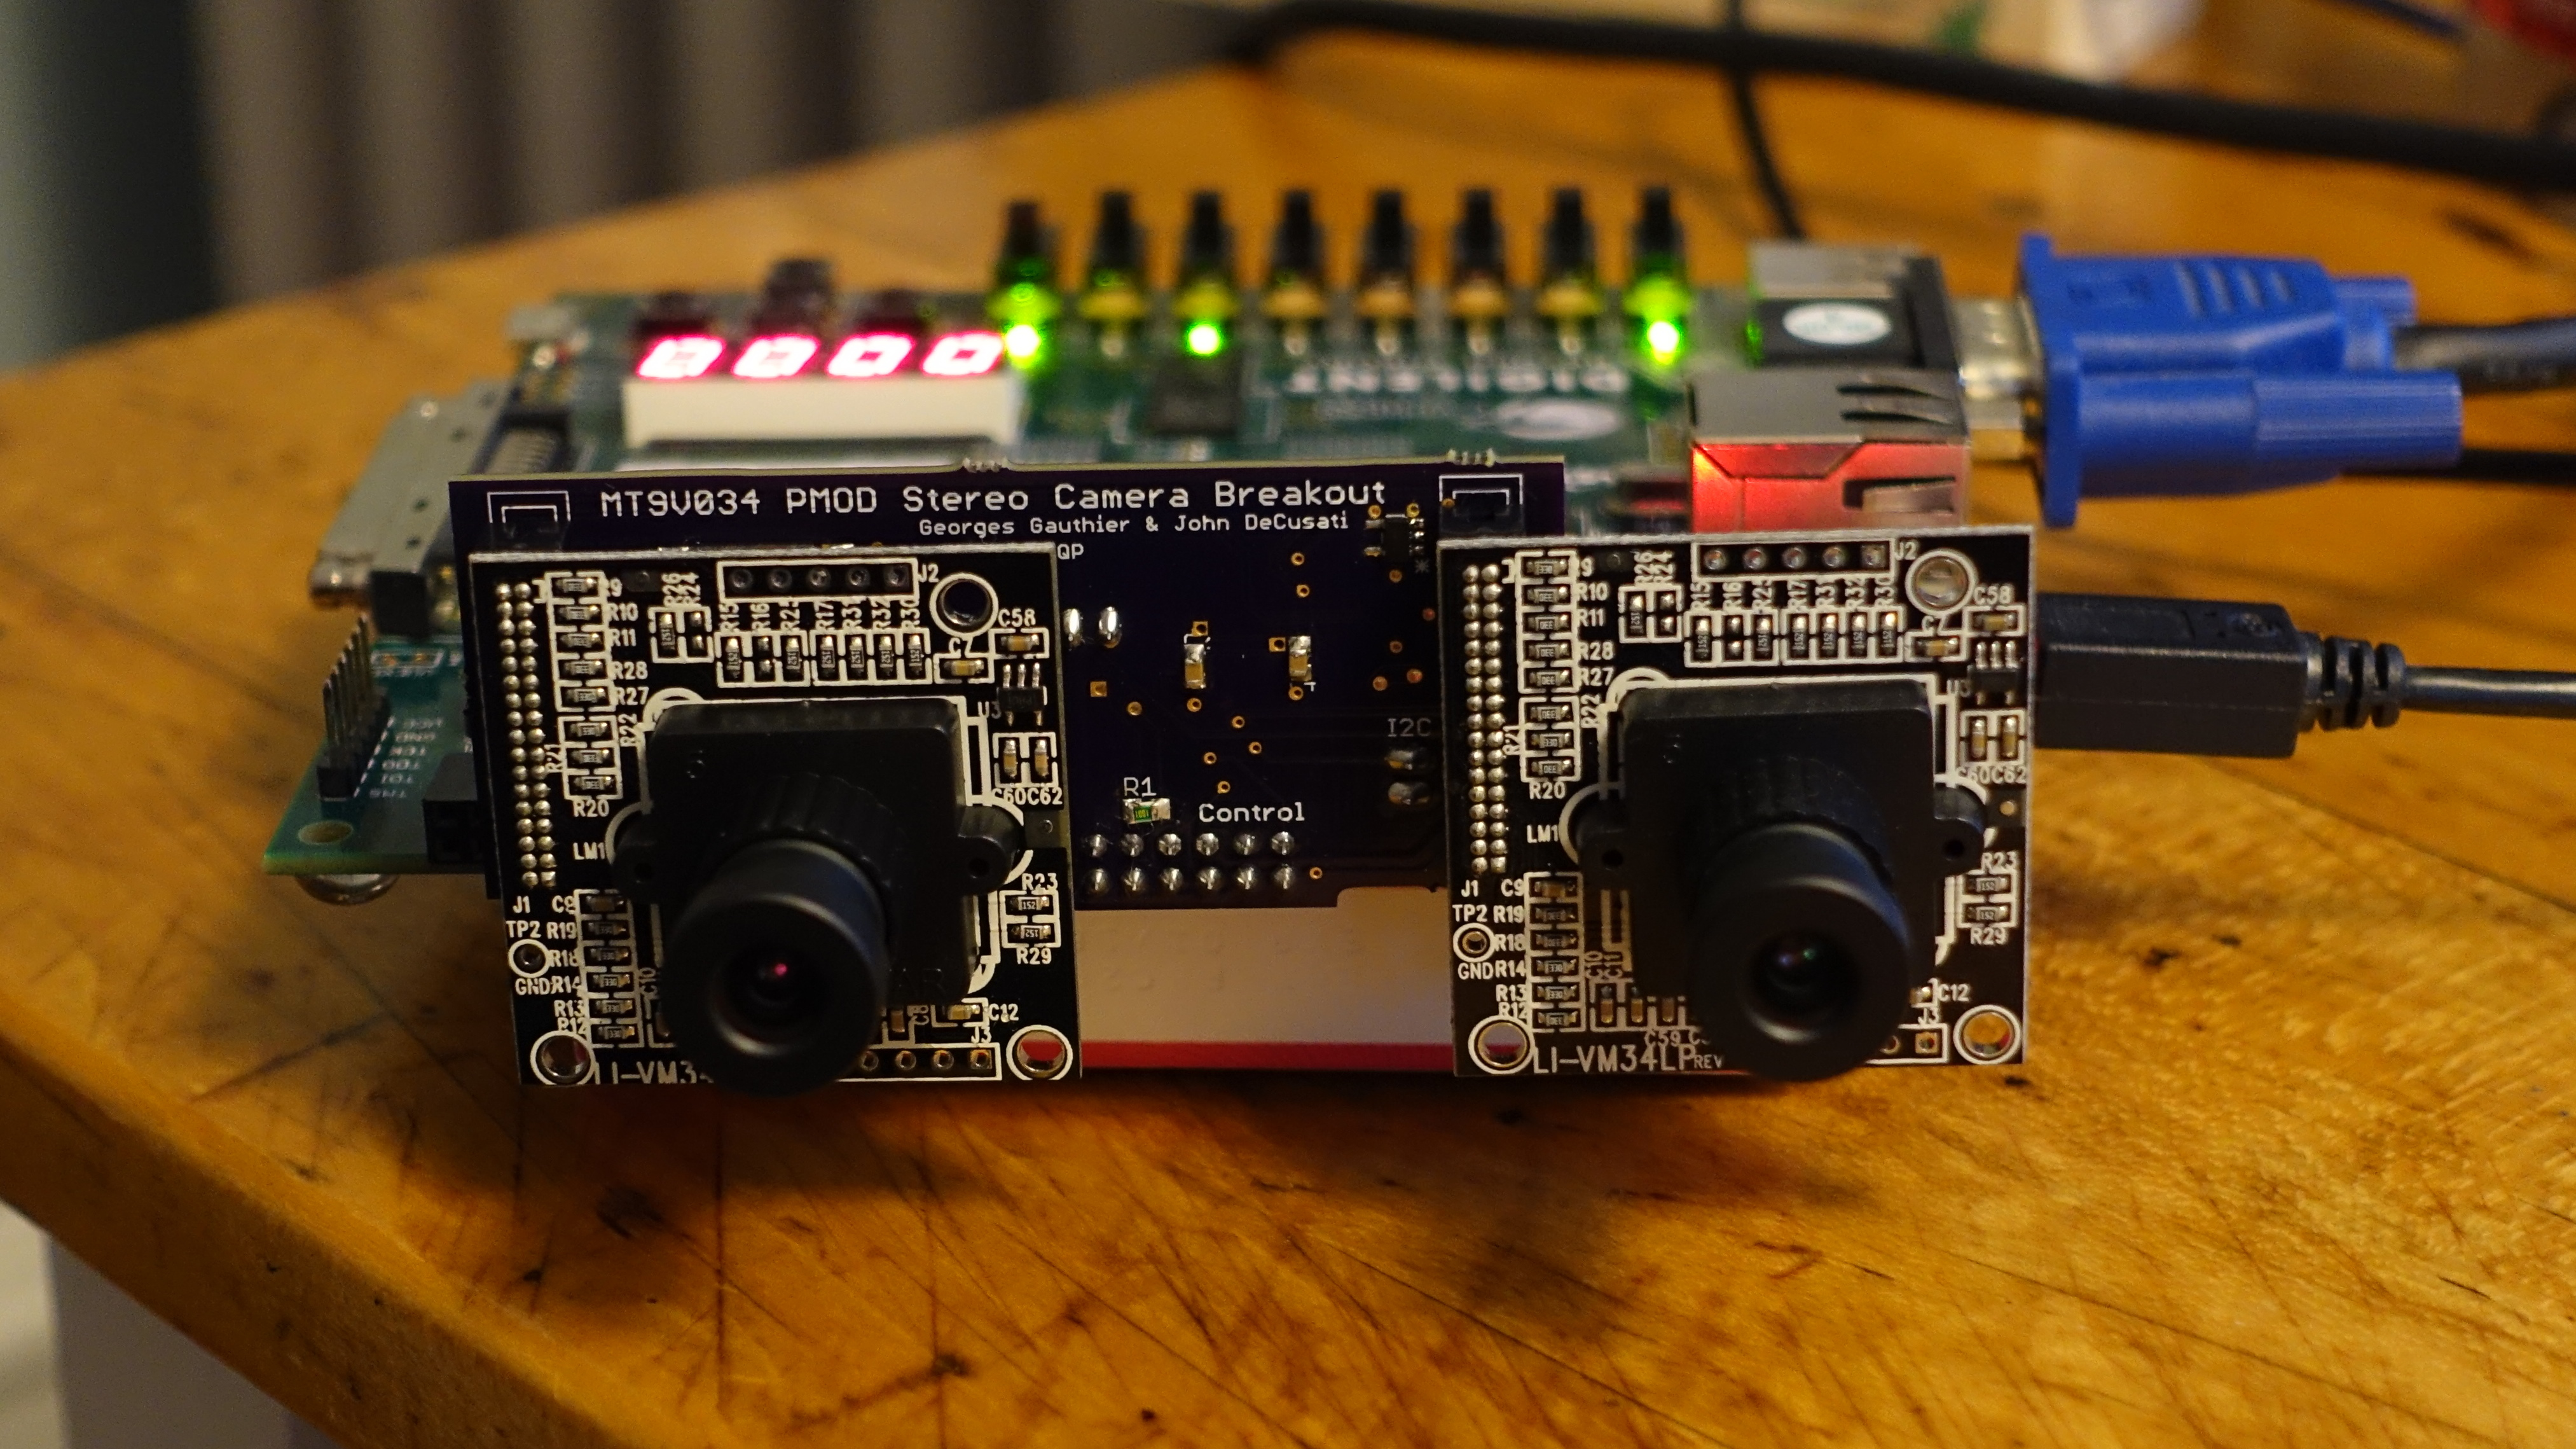
\includegraphics[width=0.8\linewidth]{stereo_breakout.JPG}
	\caption{Stereo Camera Breakout Under Test}
	\label{stereoTestSetup}
\end{figure}
\par
After manually focusing each camera using the VGA module described above, the UART transmission implementation described in Section \ref{UARTimg} was used to transmit image data from the stereo cameras to a computer for further analysis. As shown in the example image in Figure \ref{newBoardImage}, the new stereo camera setup was far less susceptible to data loss in comparison to the previous version. For further comparison, please refer back to the test image acquired using the original camera test setup shown in Figure \ref{notebookImage}.
\begin{figure}[H] 
	\centering
	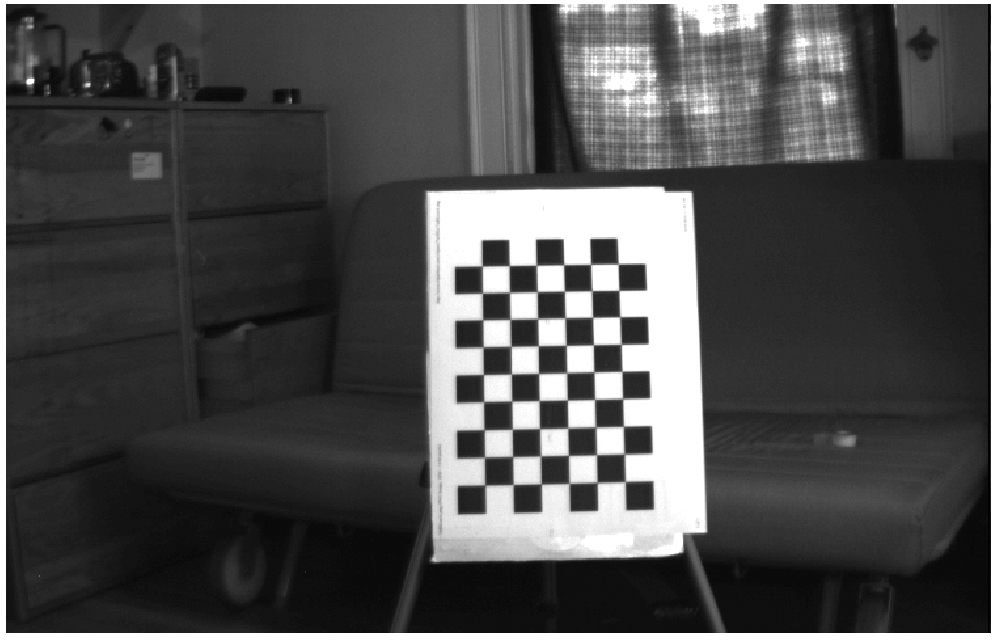
\includegraphics[width=0.8\linewidth]{cam1_image.png}
	\caption{Stereo Camera Breakout Sample Image}
	\label{newBoardImage}
\end{figure}

\subsubsection{Image Buffering}
After the camera setup was deemed working based on the results of the Nexys3 test implementation, a finalized camera controller module was created for the ZedBoard. This began with the simple implementation shown in the block diagram in Figure \ref{zedCamTest} below. This implementation contained a customized camera controller IP based around the same code used for creating the camera controller described in Appendix Item \ref{mt9v034TestCode}, with the exception that internal Block RAM was used to buffer an entire image captured from the cameras. Note that a custom AXI interface was also included in the test implementation, which allowed for the option of reading image data into the Zynq Processing System for more advanced testing and export via PS peripherals such as UART. 
\begin{figure}[H] 
	\centering
	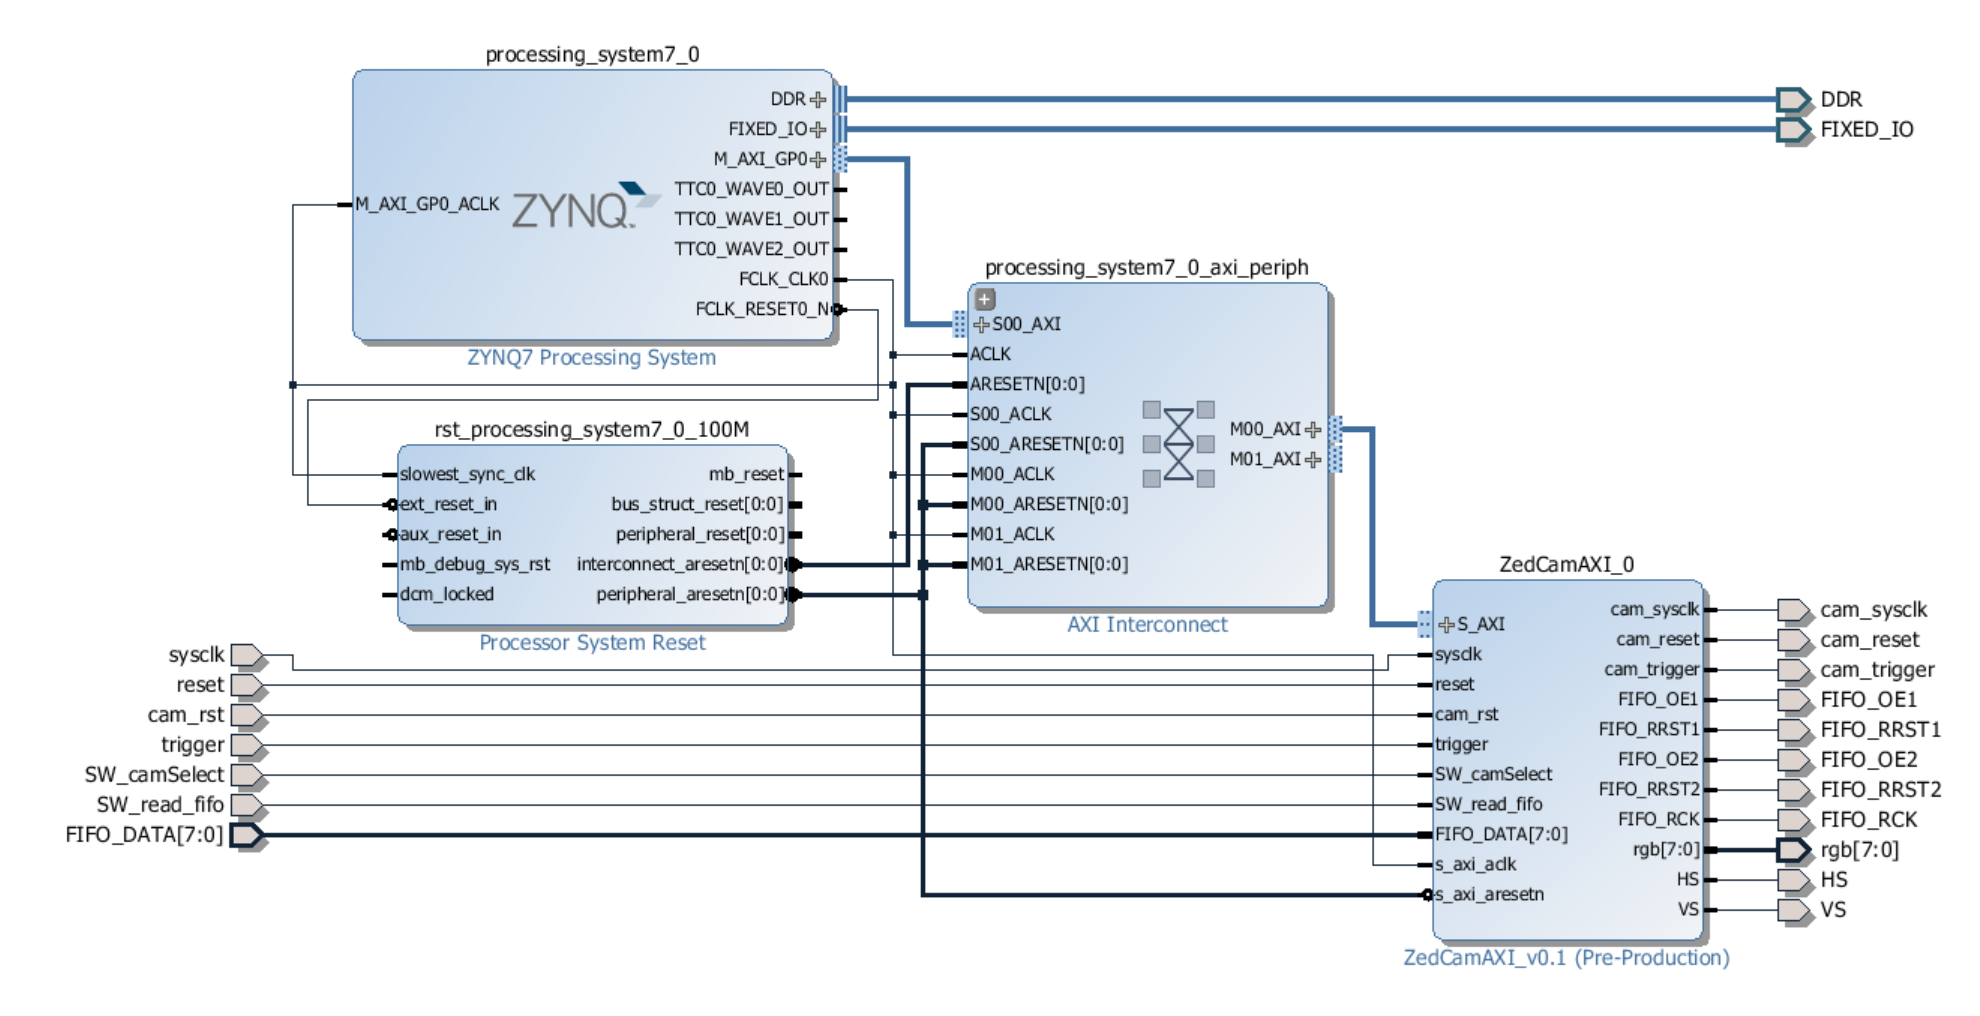
\includegraphics[width=1.0\linewidth]{zedCamTest.PNG}
	\caption{ZedBoard BRAM Camera Test Block Diagram}
	\label{zedCamTest}
\end{figure}
\par
Since a single camera image contained $8 \textrm{ bits} \times (752\times 480)$ pixels, a simple dual-port Block RAM module containing $752\times480=360960$ 8-bit addresses was created for storing the output of the AL422B FIFO reader module. Dual-port Block RAM was used to allow for external VGA logic to read from the image buffer without the need for read/write protection. Overall, the purpose of this implementation was to test the capabilities of the ZedBoard's internal BRAM for image buffering, as well as to get a simple visual confirmation that the implementation functioned properly. An example of the output from this implementation is shown in Figure \ref{bramCamTest} below. 
\begin{figure}[H] 
	\centering
	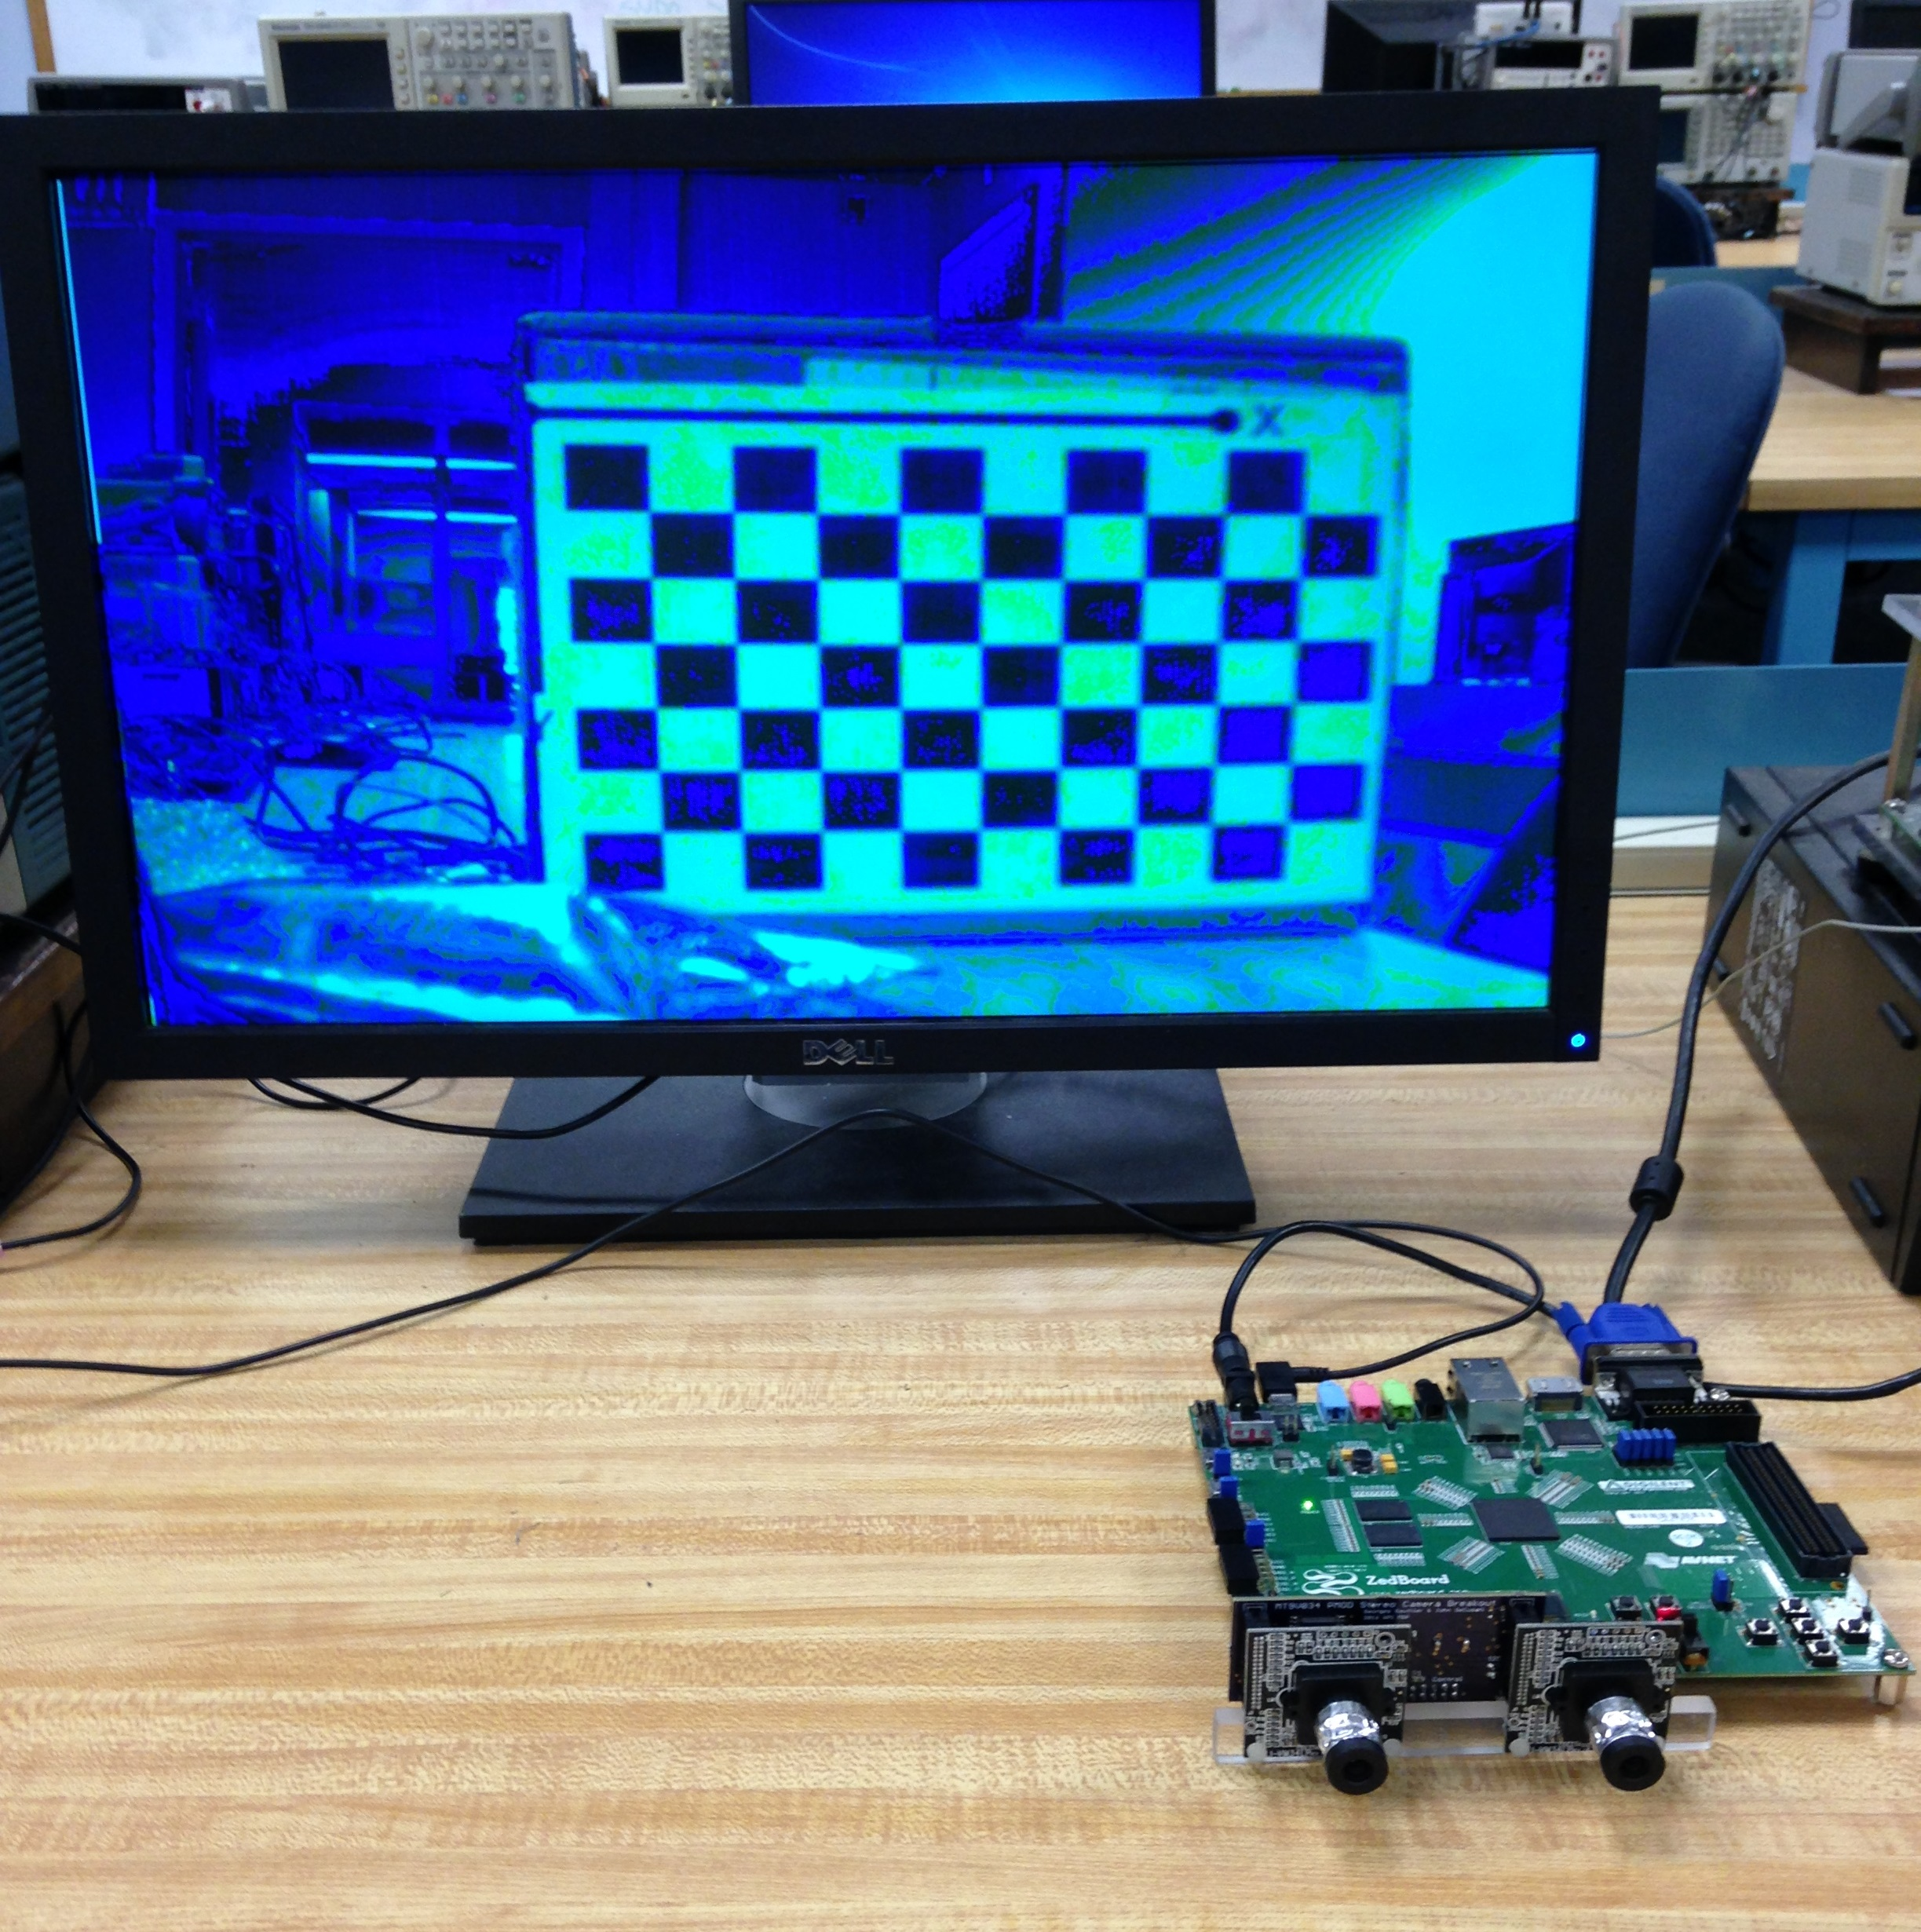
\includegraphics[width=0.6\linewidth]{bram_test.JPG}
	\caption{ZedBoard BRAM Camera Test}
	\label{bramCamTest}
\end{figure}
\par
After determining that the Zynq Processor's internal BRAM would be usable for storing image data, several tradeoffs associated with the memory requirements of buffering image data in BRAM were then addressed. 

\subsubsection{Resource Management} \label{dataman}
One major issue encountered while dealing with resource management on the ZedBoard was managing Block RAM resources. The Zynq7020 processor used on the ZedBoard contained 140 individual blocks of 36Kb BRAM, which was equivalent to 630,000 8-bit bytes of memory \cite{zynq7bram}. Although this was plenty of memory for buffering a single 752x480 camera image, three separate image buffers needed to be implemented in BRAM for this project. Two of said memory buffers were used for storing left and right camera images for processing by the disparity algorithm, and a third was used for storing a resultant output image that was then displayed via VGA.
\par
In order to address this issue, input camera imagery was centrally windowed to a resolution of 384x288 pixels, or $0.6\times{}VGA$. The output display buffer was also been reduced from WVGA (752x480) to VGA (640x480). In total, this resulted in the use of 27 36Kb Block RAM modules per input camera image, and 75 36Kb Block RAM modules for the VGA display buffer. Note that each buffer was configured using an individual Block RAM IP, and each consisted of a simple dual-port RAM with an 8-bit data length. Overall, this implementation consumed 129 out of the 140 36Kb Block RAM modules available on the ZedBoard's Zynq7020 processor, which left additional resources for use in the IMU and rangefinder implementations. 